% Тут используется класс, установленный на сервере Papeeria. На случай, если
% текст понадобится редактировать где-то в другом месте, рядом лежит файл matmex-diploma-custom.cls
% который в момент своего создания был идентичен классу, установленному на сервере.
% Для того, чтобы им воспользоваться, замените matmex-diploma на matmex-diploma-custom
% Если вы работаете исключительно в Papeeria то мы настоятельно рекомендуем пользоваться
% классом matmex-diploma, поскольку он будет автоматически обновляться по мере внесения корректив
%

% По умолчанию используется шрифт 14 размера. Если нужен 12-й шрифт, уберите опцию [14pt]
\documentclass[14pt]{matmex-diploma}
%\documentclass[14pt]{matmex-diploma-custom}
\usepackage{mathtools}      % матрицы 
\usepackage{amsfonts, amsmath}
\usepackage{multicol,caption,float, subfig} % картинки

\hyphenpenalty=10000    % пенальти на переносы (max)
\sloppy % режим разрешает разрежать строки
\widowpenalty=4000 % пенальти на висячие строки в конце абзаца  
\clubpenalty=4000 % пенальти на висячие строки в начале абзаца

\usepackage{mathtext}
%\usepackage[T2A]{fontenc}
%\usepackage[utf8]{inputenc}
%\usepackage[russian]{babel}




\begin{document}
% Год, город, название университета и факультета предопределены,
% но можно и поменять.
% Если англоязычная титульная страница не нужна, то ее можно просто удалить.
\filltitle{ru}{
    faculty = {Математическое обеспечение и администрирование информационных систем},
    chair              = {Информационно-аналитические системы},
    title              = {Методы машинного обучения в задаче предсказания погоды},
    % Здесь указывается тип работы. Возможные значения:
    %   coursework - Курсовая работа
    %   diploma - Диплом специалиста
    %   master - Диплом магистра
    %   bachelor - Диплом бакалавра
    type               = {coursework},
    position           = {студента},
    group              = 646,
    author             = {Волжина Елена Григорьевна},
    supervisorPosition = {доцент},
    supervisor         = {Михайлова Е.\,Г.},
%    reviewerPosition   = {}, TODO
%    reviewer           = {Ганьшин А.\,В.},
    chairHeadPosition  = {профессор},
    chairHead          = {Новиков Б.\,А.},
    university         = {Санкт-Петербургский Государственный Университет},
    city               = {Санкт-Петербург},
    year               = {2017}
}
\filltitle{en}{
    faculty = {Software and Administration of Information Systems},
    chair              = {Analytical Information Systems},
    title              = {Machine learning methods in weather prediction problem},
    type               = {coursework},
    author             = {Elena Volzhina},
    supervisorPosition = {associate professor},
    supervisor         = {Elena Mikhaylova},
%    reviewerPosition   = {assistant},
%    reviewer           = {Alexander Ganshin},
    chairHeadPosition  = {professor},
    chairHead          = {Boris Novikov},
    year               = {2017}
}


\maketitle
\tableofcontents


% У введения нет номера главы
% ВВЕДЕНИЕ
\section*{Introduction}
С ростом производительности вычислительных систем, объемов накопленных данных об окружающем мире и опыта в их обработке находятся всё новые и новые области для применения анализа данных. Одной из таких областей сегодня является и прогнозирование погодных условий и в целом состояния атмосферы.

With the growth of computing performance, the volume of accumulated data about the surrounding environment and experience in processing such amounts of data, more and more areas appear to apply data analysis. One of these areas today is the forecasting of weather conditions and the overall state of the atmosphere.

Прогнозы погоды полезны как обычным людям для принятия бытовых решений, так и в более серьезных областях: в авиации, судоходстве, а также в сельском хозяйстве. Большую пользу знания о погоде в будущем могут принести и бизнесу, в особенности сезонному, в котором спрос на услуги или возможность проводить работы сильно зависит от погоды.

Weather forecasts are useful both for ordinary people to make household decisions, and in more serious areas: aviation, shipping, and agriculture.  A great benefit of knowledge about the weather in the near future can bring and business, especially seasonal, in which the demand for services or the ability to carry out work is highly dependent on the weather.

В Яндексе для прогноза погоды используется технология Метеум, комбинирующая прогнозы от нескольких поставщиков и другие данные с помощью методов машинного обучения, а именно градиентного бустинга над решающими деревьями. Модель, полученная таким образом, улучшает качество прогноза относительно каждого из поставщиков.

Yandex.Weather forecasting technology is named Meteum and combines the forecasts from several suppliers and other data using machine learning techniques, namely gradient boosting on decision trees. The model obtained in this way improves the quality of the forecast of each of the suppliers.

В рамках этой работы я добавляла к используемым моделью данным информацию о погоде в интересующей нас области в тот момент, когда мы вычисляем свой прогноз. Это может улучшить предсказания для ближайшего будущего, так как оно естественным образом зависит от настоящего.

In this work, I added to the data used by model information about the weather in the specific area at the moment we calculated forecast. This can improve predictions for the near future because it naturally follows from the present.

% численный прогноз погоды https://ru.wikipedia.org/wiki/Численный_прогноз_погоды
% https://ru.wikipedia.org/wiki/Прогноз_погоды 


% ОБЗОР ЛИТЕРАТУРЫ?
\section{Существующие решения -- Study area}

% про модели, СПИСОК ЛИТЕРАТУРЫ http://method.meteorf.ru/publ/tr/tr359/tolstih.pdf

% на основе lynch2008origins -- история прогнозов
% http://www.mbureau.ru/articles/istoriya-razvitiya-modeley-prognozirovaniya-pogody
% https://habrahabr.ru/post/179687/ -- практически то же, что предыдущее

% от Саши: \cite{васильев2008прогноз} -- познавательный обзор

Наблюдения за погодой и попытки её предсказывать ведутся с тем или иным успехом уже несколько веков. Изначально прогнозы делались на основе опыта наблюдений и примет, но уже в XIX веке с развитием гидродинамики и термодинамики появляются первые математические инструменты для прогнозов. 

Weather observations and attempts to predict it are conducted with some success for several centuries. Initially, forecasts were made on the basis of observation experience and weather sightings, but in the 19th century with the development of hydrodynamics and thermodynamics, the first mathematical tools for forecasts appear.

К концу XIX века научное сообщество располагало инструментами для исследования поведения газов, законами, описывающими это поведение, а также представлением о крупных системах, обуславливающих состояние атмосферы и, как следствие, погоду в конкретной точке. Были сформулированы идеи о решении системы уравнений с заданными начальными условиями для предсказания погоды в будущем.

By the end of the 19th century, the scientific community had tools to study the behavior of gases, physical laws describing this behavior, as well as the initial understanding of large systems that determine the state of the atmosphere and, as a consequence, the weather at a particular point. Ideas for solving a system of equations with given initial conditions for predicting the weather in the future were formulated.

В начале XX века Льюис Фрай Ричардсон составил систему уравнений, описывающих процессы, по которым меняется состояние атмосферы. Подставив в качестве начальных условий текущее состояние атмосферы можно было решить систему методом конечных разностей и получить прогноз изменения атмосферного давления\cite{lynch2008origins}. При этом задавать начальные условия требовалось с большой точностью, так как даже небольшая погрешность в них приводила к большим изменениям в результате расчётов. Также значительной проблемой была вычислительная сложность процесса, она делала невозможным сколько-нибудь оперативный прогноз погоды в реальных условиях.

At the beginning of the 20th century Lewis Fry Richardson composed a system of equations describing the processes by which the state of the atmosphere changes. Substituting the current state of the atmosphere as initial conditions, it was possible to solve the system by the method of finite differences and obtain a prediction of atmospheric pressure changes\cite{lynch2008origins}. At the same time, it was necessary to set initial conditions with great accuracy, since even a small error in them led to large changes in the result of calculations. Also, a significant problem was the computational complexity of the process, it made it impossible to any operational weather forecast in current conditions.

Во второй половине XX века появляются всё новые сведения об атмосферных процессах, уточняющие точность моделирования, а также вычислительные ресурсы и технологии, необходимые для регулярного решения подобных систем в разумных временных рамках. Численное моделирование крупномасштабных явлений в атмосфере значительно улучшилось благодаря информации с искусственных спутников Земли\cite{васильев2008прогноз}.

In the second half of the 20th century appears new information about atmospheric processes, improving the accuracy of modeling, as well as the computing resources and technologies necessary for the regular solution of such systems in a reasonable time frame. Numerical simulations of large-scale atmospheric phenomena have been significantly improved because of the information from artificial earth satellites\cite{vassiliev2008prognoz}.


\subsection{Классические методы -- Classical methods}

% https://en.wikipedia.org/wiki/Numerical_weather_prediction
% https://en.wikipedia.org/wiki/Global_Forecast_System
% 

Классический подход к задаче прогноза погоды включает в себя несколько компонентов. В основе всего лежит сбор данных: как долгосрочные наблюдения о температуре, осадках и прочих параметрах в конкретной местности, так и регулярные замеры с помощью разнообразной техники: приборов, установленных на наземных метеостанциях, метеорологических зондов и даже метеорологических спутников. Далее в дело вступают математические модели атмосферы, настроенные с помощью собранных данных. В этих моделях уравнения гидрогазодинамики описывают процессы в атмосфере, которые влияют на интересующие нас величины, а подставив в качестве параметров реальные данные о состоянии атмосферы в данный момент мы можем получить прогноз её состояния через некоторое время.

The classical approach to the problem of weather forecasting includes several components. Data collection is in a basis of the solution: both long-term observations of temperature, precipitation and other parameters in a specific area, and regular measurements using a variety of techniques: devices installed at ground weather stations, meteorological probes and even meteorological satellites. Next, the mathematical models of the atmosphere, configured with the collected data, come into play. In these models, the equations of hydrogasdynamics describe processes in the atmosphere that affect the values of interest to us. Substituting as parameters for these models real data on the state of the atmosphere at the moment we can get a forecast of its state after a while.

Модели атмосферы можно разделить на \textit{глобальные}, покрывающие всю планету, и \textit{региональные}, описывающие ограниченную территорию. Первые более универсальны, зато вторые могут давать лучшее качество для своих областей за счет более тонкой настройки и высокого расширения. Сами прогнозы можно разделить на группы по времени, на которое мы смотрим в будущее: \textit{краткосрочные} (до 72 часов), \textit{среднесрочные} (от 72 часов до 10 суток) и \textit{долгосрочные} (более 10 суток).

[TODO: курсивы] Atmospheric models can be divided into global, covering the entire planet, and regional, describing a limited area. The first is more universal, but the second can give the best quality for their areas at the expense of more fine-tuning and of high expansion. The forecasts themselves can be divided into groups by the time we look to the future: short-term (up to 72 hours), medium-term (from 72 hours to 10 days) and long-term (more than 10 days).

% дальше инфа от Димы в баре
Построение и обновление математических моделей атмосферы очень трудозатратно и требует проведения большого количества различных экспериментов, поэтому из-за постоянных изменений климата все использующиеся модели являются в большей или меньшей степени устаревшими. Помимо этого, так как физика многих процессов в атмосфере еще недостаточно изучена, у всех моделей есть те или иные погрешности в прогнозировании, при этом зачастую эти погрешности имеют постоянную природу: например, одна из моделей может завышать температуру, а другая -- занижать давление в горах.

Building and updating mathematical models of the atmosphere is very laborious and requires a large number of different experiments, so due to the constant changes in the climate all used models are more or less obsolete. In addition, since the physics of many processes in the atmosphere is not yet sufficiently studied, all models have certain errors in forecasting. Often these errors have a constant nature: for example, one of the models may overestimate the temperature, and the other --[TODO] to underestimate the pressure in the mountains.

Учитывая объемы информации, человеку сложно найти эти шаблоны в ошибках моделей. Но благодаря современным статистическим методам и вычислительным мощностям этот процесс можно автоматизировать. Именно эта идея лежит в основе технологии Метеум, которая используется для прогноза погоды в Яндексе. По накопленным данным о прогнозах разных моделей и фактической погоде в моменты, на которые делались эти прогнозы, можно построить модель, корректирующую прогнозы поставщиков и улучшающую качество итогового прогноза.

Due to the large amount of information, it is difficult for a person to find these patterns in model errors. But thanks to modern statistical methods and computing power, this process can be automated. This idea is the basis of technology Meteum, which is used to forecast the weather in Yandex. Based on accumulated data on forecasts of different models and actual weather at the moments for which forecasts were made, it is possible to build a model that corrects supplier forecasts and improves the quality of the final forecast.


\subsection{Машинное обучение, технология Метеум -- Machine learning, Meteum technology}
% метеум https://habrahabr.ru/company/yandex/blog/271725/
% наукаст https://habrahabr.ru/company/yandex/blog/317626/
% техническая часть наукаста https://habrahabr.ru/company/yandex/blog/328158/
% новая архитектура https://habrahabr.ru/company/yandex/blog/343518/

\textit{Машинным обучением} называют подход к решению задач, заключающийся в анализе большого количества накопленных наблюдений с целью найти в них ранее неизвестные зависимости. Нередко такие зависимости сложно или невозможно (например, в силу недоступности информации о части факторов) описать формально, но благодаря статистическому подходу их можно приблизить с достаточным для практического применения качеством\cite{bishop}.

Machine learning is the approach to solving problems, which consists in analyzing a large number of accumulated observations in order to find previously unknown dependencies. Often, such dependencies are difficult or impossible to describe formally (for example, due to the unavailability of information about some factors), but thanks to a statistical approach, they can be approached with sufficient quality for practical use\cite{bishop}.

В задаче предсказания погоды удобно использовать методы \textit{обучения с учителем} -- они применяются, когда на каждое наблюдение, описанное вектором факторов, имеется "правильный ответ". Среди них выделяют методы \textit{классификации}, когда ответом является метка из конечного множества (например, если предсказывается наличие осадков или их тип), и методы \textit{регрессии}, в этом случае ответ -- непрерывная величина (например, температура или количество осадков в миллиметрах).

[todo: курсивы] In the problem of weather prediction, it is convenient to use supervised learning methods -- they are used when each observation described by the feature vector has a "correct answer". These include classification methods, where the answer is a label from a finite set (for example, if the presence of precipitation or its type is predicted), and regression methods, in which case the answer is a continuous value (for example, temperature or precipitation in millimeters).

В качестве примера можно упомянуть The Weather Company, которая для подсчёта прогноза погоды комбинирует информацию из более чем 150 источников данных с помощью машинного обучения\cite{ibm_weather}.

As an example we can mention The Weather Company, which combines information from more than 150 data sources using machine learning for the calculation of forecast\cite{ibm_weather}.

Сервис Яндекс.Погода использует для прогноза погоды технологию Метеум. На основе накопленных данных, которые будут описаны подробнее далее, составляются отдельные модели машинного обучения для интересующих нас параметров: температуры, давления, скорости и направления ветра, а также типа облачности и осадков. Важно уточнить, что температура предсказывается не сама по себе, а как разница между температурой и климатическими данными -- усредненными показаниями за десятки лет для этого времени года. Это позволяет частично избавиться от сезонности в изменениях температуры.

Yandex.Weather uses weather technology Meteum. Based on the accumulated data, which will be described in more detail below, separate machine learning models for the parameters we are interested in are compiled: temperature, pressure, wind speed and direction, as well as the type of cloudinesses and precipitation. It is important to clarify that temperature is not predicted by itself, but as the difference between temperature and climate data -- averaged over many years for this time of year. This allows us to get rid of seasonality in temperature changes.

Для обучения в числе прочего используются данные, вычисляемые через классические модели прогнозирования. Сравнивая эти прогнозы с фактическими показаниями, модель находит зависимости целевой переменной от прогнозов разных показателей (например, для осадков кроме, собственно, прогнозов осадков, важными факторами оказываются также прогнозы облачности), а также учится исправлять упомянутые выше погрешности разных моделей.

Training uses, among other things, data calculated from classical forecasting models. Comparing these forecasts with the actual values, the model finds the dependence of the target variable on the forecasts of different indicators (for example, for prediction of precipitation except precipitation forecasts itself, important factors are also cloud forecasts), and learns to correct the aforementioned constant errors of different models.

В рамках данной работы будет проверена гипотеза о том, что полезной информацией для предсказаний погоды в ближайшем будущем окажется состояние погоды на данный момент. Для этого будут использоваться показания с одной или двух ближайших метеорологических станций.

In this paper will be tested the hypothesis that weather conditions at the moment will be useful information for predicting weather in the near future. The readings from one or two nearest meteorological stations will be used for this purpose.


\begin{figure}
\centering
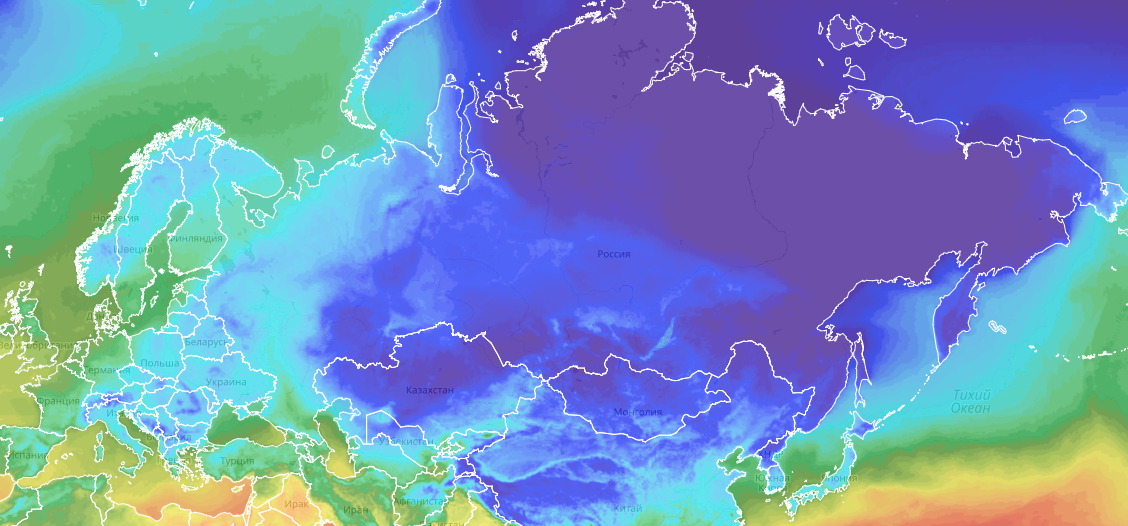
\includegraphics[width=\linewidth]{images/map_coursework.png}
\caption{Карта температуры на Яндекс.Погоде -- Temperature map at Yandex.Weather}
\label{fig:map}
\end{figure}



% МЕТОДОЛОГИЯ
\section{Методология -- METHODS}
Прежде чем приступать к экспериментам, следует разобраться с данными, которыми мы располагаем, решить, как мы будем собирать обучающую выборку с известными ответами и готовить её к использованию. Далее нужно выбрать метод для поиска решающей функции, которая бы приближала правильные ответы, находя зависимости в данных. Также необходимо определить метрики, с помощью которых будет приниматься решение, успешным считать эксперимент или нет. После этого можно будет приступать к основной задаче: добавить к обучающей выборке данные о текущих погодных условиях в месте, для которого рассчитывается прогноз; попробовать обучить на расширенных данных модель для предсказания температуры; оценить по метрикам улучшение.

Before the start of experiments, we should overview the data we have, decide how we will collect the training sample with known answers and prepare it for use. Next, we need to choose a method to find the decisive function that would approximate the correct answers by finding dependencies in the data. It is also necessary to determine the metrics by which we can consider the experiment as successful or not. After that, we will be able to start the main task: to add to the training sample information about current weather conditions in the place for which the forecast is calculated; to try to teach the model for temperature prediction on extended data; and finally to estimate improvement on metrics.


\subsection{Данные для обучения -- Dataset for learning}
При составлении прогноза мы располагаем множеством данных, полученных от поставщиков или вычисленных самостоятельно. Можно выделить несколько групп этих данных:

When we make a prediction, we have a lot of data from vendors and also data calculated by us. We can select multiple types of these data:

\begin{enumerate}
% GFS (США), ECMWF (Англия), JMA (Япония), CMC (Канада), EUMETSAT (Франция), Earth Networks (США) 

    \item \textit{прогнозы погоды}, сделанные при помощи математического моделирования физических процессов в атмосфере; в числе поставщиков следующие глобальные модели: Global Forecast System (GFS \cite{saha2006ncep}), Japan Meteorological Agency (JMA), European Centre for Medium-Range Weather Forecasts (ECMWF \cite{persson2001user}), Canadian Meteorological Centre (CMC). Также на серверах Яндекс.Погоды рассчитывается региональная модель для собственных прогнозов -- Weather Research and Forecasting Model (WRF). У разных моделей могут различаться частота расчётов, координатная сетка, а также набор параметров в прогнозе, это необходимо учитывать при сборе обучающей выборки;

    \item \textit{фактические данные} о погоде, снятые на метеостанциях по всему миру с помощью статических приборов и метеозондов. Используются станции из сети Всемирной метеорологической организации;
    
    \item \textit{климатические данные}, посчитанные на основе десятков лет наблюдений метеостанций;

    \item \textit{радарные данные} об осадках и облачности, \textit{спутниковые снимки}.
\end{enumerate}


TODO: курсивы 
\begin{enumerate}
    \item weather forecasts made using mathematical modeling of physical processes in the atmosphere; among the suppliers are the following global models: Global Forecast System (GFS \cite{saha2006ncep}), Japan Meteorological Agency (JMA), European Centre for Medium-Range Weather forecast (ECMWF \cite{persson2001user}), Canadian Meteorological Centre (CMC). Also on Yandex.Weather servers for the most interesting for us regions is calculated the regional model -- Weather Research and Forecasting Model (WRF). Different models may have different calculation frequency, coordinate grid, as well as a set of parameters in the forecast, this should be taken into account when collecting the training sample;

    \item actual weather data from weather stations around the world obtained using static instruments and meteoprobes. Stations from the World Meteorological Organization (WMO) network are used;
    
    \item climate data calculated on the basis of decades of observations of weather stations;

    \item radar data for precipitation and cloud cover, the satellite images.
\end{enumerate}

Чтобы применять на этих данных какие-либо алгоритмы машинного обучения, нужно очистить их от выбросов и шума, привести всех поставщиков к единой координатной сетке и собрать обучающую выборку. В момент, когда мы делаем прогноз, мы можем использовать полученные ранее прогнозы от поставщиков, статистические данные о климате, а также информацию о погоде в интересующей нас точке в данный момент (или, с учётом задержек, в недавнем прошлом).

To use any machine learning algorithms on this data, we need to clean it from outliers and noise, bring all suppliers to a single coordinate grid, and collect a training dataset. At the time we make the forecast, we may use previously obtained forecasts from suppliers, climate statistics as well as weather information at the point of interest to us at the moment (or, to take into account delays, in the recent past).

Нам потребуется множество наблюдений $X = \{x_i = (f^1_{i}, \cdots, f^M_i), i \in \overline{1..N}\}$, элементы которого соответствуют векторам признаков, полезных для предсказывания в текущий момент $gentime$ состояния погоды на момент в будущем $time$. Например, в числе этих признаков будут прогнозы различных погодных параметров: температуры, влажности, скорости и направления ветра, осадков и облачности. Эти прогнозы должны быть сделаны на время, близкое к интересующему нас $time$, при этом при сборе обучающей выборки важно не заглядывать в будущее, то есть время генерации этих прогнозов поставщиками должно быть не позже, чем $gentime$ (а с учётом задержек при передаче данных лучше брать прогнозы, сделанные еще раньше). Помимо множества наблюдений $X$ нам понадобится множество истинных значений $y = \{y_i, i \in \overline{1..N}\}$, в нашем случае это разница температуры, которая была получена с метеостанции в момент $time$ (на это время мы делали прогноз), с усредненной за много лет температурой в этот день и в это время: $temperature\_delta = fact\_temperature - climate\_temperature$.


We need a set of observations $X = \{x_i = (f^1_{i}, \cdots, f^M_i), i \in \overline{1..N}\}$, the elements of which correspond to feature vectors useful for predicting the current ($gentime$) weather conditions at the moment in the future ($time$). For example, these indicators will include forecasts of various weather parameters: temperature, humidity, wind speed and direction, precipitation and cloud cover. These forecasts should be made for a time close to the $time$ we are interested in, while it is important not to look into the future when collecting a training sample, that is, the time of generation of these forecasts by suppliers should be no later than $gentime$ (and taking into account delays in the transfer of data, it is better to take forecasts which were made earlier). In addition to the set of observations $X$ we need a set of true values $y = \{y_i, i \in \overline{1..N}\}$, in our case, it is the temperature difference that was obtained from the weather station at the time $time$ (for this time we did the forecast), with an average temperature for many years on this day and at this time: $temperature\_delta = fact\_temperature - climate\_temperature$.


\subsection{Решающие деревья и градиентный бустинг -- Decision trees and gradient boosting}

Для проведения экспериментов по прогнозу температуры на основе имеющихся данных, был выбран алгоритм \textit{градиентного бустинга над решающими деревьями}. Использовалась реализация этого алгоритма под названием Матрикснет, разработанная и использующаяся в компании Яндекс.

To conduct experiments on the temperature prediction based on the available data, the gradient boosting algorithm over the deciding trees was chosen. The implementation of this algorithm, called Matrixnet, was developed and used by Yandex.

\textit{Решающее дерево} -- это алгоритм предсказания, описывающийся бинарным деревом, у которого каждой внутренней вершине $v$ поставлен в соответствие некоторый предикат $\beta_v: X \to \{0, 1\}$, а каждому листу соответствует метка с ответом алгоритма\cite{bishop}. После обучения применяется дерево следующим образом: для фиксированного $x \in X$ начинаем с корневой вершины ($v_{root}$). Вычисляем значение $\beta_{v_{root}}(x)$. Если получили $0$, переходим в левого потомка, если $1$ -- в правого. Продолжаем до тех пор, пока не окажемся в листе, метку которого и возвращаем в качестве ответа.

\textit{Decision tree} is the machine learning algorithm, described by binary tree in which each internal vertex $v$ corresponds to some predicate $\beta_v: X \to \{0, 1\}$, and each leave node corresponds to the label with the answer of the algorithm\cite{bishop}. After learning, the tree is used as follows: for a fixed $x \in X$ we start from the root vertex ($v_{root}$). Then we calculate the value $\beta_{v_{root}} (x)$. If we get $0$, we pass in left descendant, if $1$ -- in right one. Continuing until we reach the leave, its label will be returned as the response of algorithm for $x$.

\textit{Градиентный бустинг} -- алгоритм, с помощью которого по обучающим данным последовательно строится композиция из простых алгоритмов предсказания, причём каждый следующий алгоритм в композиции стремится уменьшить ошибку, которую даёт уже накопленный ансамбль. Такой метод построения называют \textit{жадным}, так как он вместо попытки сразу найти оптимальное решение, идёт к нему итеративно, делая на каждом шаге локально-оптимальный выбор\cite{friedman2001greedy}.

Gradient boosting is an algorithm with the help of which, according to the training data, the composition of simple prediction algorithms is sequentially constructed, and each following algorithm in the composition seeks to reduce the error that the already accumulated ensemble gives. This method of construction is called \textit{greedy}, because instead of trying to find the optimal solution at once, it goes to it iteratively, making at each step a locally optimal choice\cite{friedman2001greedy}.

Градиентный бустинг позволяет из простых предсказательных моделей, не приносящих хороших результатов при самостоятельном использовании, получить композицию, хорошо приближающую целевую функцию. При этом модель оказывается устойчивой к переобучению и эффективной в применении (так как простые элементы композиции можно быстро вычислить параллельно) \cite{FRIEDMAN2002367}.

Gradient boosting allows to obtain a composition of simple predictive models, which do not bring good results when used independently, but this composition approximates the target function much better. In this case, the model is resistant to overfitting and is effective in application (since simple elements of the composition can be calculated quickly in parallel) \cite{FRIEDMAN2002367}.



\subsection{Метрики -- Metrics}
Для ответа на вопрос, улучшают изменения прогноз или ухудшают, необходимо выбрать метрики, с помощью которых в дальнейшем можно будет сравнивать качество разных моделей.

To answer the question whether the changes improve the forecast or worsen, we need to select metrics that can be used to compare the quality of different models.

Стандартной метрикой в задаче регрессии (предсказания действительного числа) является \textit{квадратный корень из среднеквадратичной ошибки} (Root Mean Square Error, RMSE). Он показывает, как сильно в среднем прогнозы модели отличаются от фактических данных. Для столбца фактических показаний $y$ и столбца ответов модели $\hat{y}$ значение этой метрики вычисляется следующим образом:
        $$RMSE(y, \hat{y}) = \sqrt{\sum^{n}_{i=1}{(y_i - \hat{y_i})^2}}$$

The standard metric in the regression problem (real number prediction) is \textit{root-mean-square error} (RMSE). It shows how much on average model forecasts differ from actual data. For the $y$ actual reading column and the $\hat{y}$ model response column, the value of this metric is calculated as follows:
        $$RMSE (y, \hat{y}) = \sqrt{\sum^{n}_{i=1}{(y_i - \hat{y_i})^2}}$$

%Помимо усредненной ошибки нам также хотелось бы понимать, как часто формула ошибается достаточно сильно для того, чтобы вызвать недоумение пользователя сервиса. В качестве порогового значения было выбрано отклонение прогноза от фактической температуры на 5 градусов. Получаем метрику
%        $$Errors_5(y, \hat{y}) = \sum^{n}_{i=1}{[|y_i - \hat{y_i}| > 5]},$$
%    \indent где $[x] = 1\text{, если } x \text{ верно, иначе } 0$.

Чтобы значения метрик объективно отражали качество моделей, нужно считать их на новых для модели примерах. В нашем случае достаточно разделить обучающую выборку на два непересекающихся подмножества ($X_{train}$ и $X_{test}$): наблюдения до определенной даты и после неё, на первом подмножестве обучить модель, а на втором вычислить метрики. Так мы не только будем проверять модель на примерах, которые не встречались ей при обучении, но и не дадим ей подглядывать в будущее (это плохо, так как погоду в последовательные моменты времени нельзя считать независимой).  

To ensure that the metric objectively reflects the quality of the model, we need to calculate it on the new examples for the model. In our case, it is enough to divide the training sample into two disjoint subsets ($X_{train}$ and $X_{test}$): observations before and after a certain date. On the first subset we can train the model, and on the second -- calculate metrics. That way we will not only check the model on the examples that it had not met during training, but also will not give her a peek into the future (this is bad, because the weather in successive moments of time can not be considered as independent -- in machine learning it's called data leak).

%Если бы мы делили $X$ не по дате, а, например, случайным образом, то рисковали бы получить чересчур оптимистичные метрики, ведь модель оценивалась бы по работе на датах, для которых она уже знала gjckt
% Вдобавок таким образом мы получаем оценку положения дел, приближенную к проду

% ЭКСПЕРИМЕНТЫ
\section{Эксперименты -- EXPERIMENTS}

Для улучшения прогноза погоды в ближайшем будущем было опробовано добавление в обучающую выборку данных о текущей погоде в области, для которой делается прогноз. Обученная модель сравнивалась с использующейся в данный момент в Яндекс.Погоде. Целевой переменной была разница между фактической температурой и средней для этих местности и времени ($temperature\_delta = fact\_temperature - climate\_temperature$).

To improve the weather forecast in the near future, we tested adding current weather data in the area for which the forecast is made to the training sample. The trained model was compared with the one currently used in Yandex.Weather. The target variable was the difference between the actual temperature and the average for the area and time ($temperature\_delta = fact\_temperature - climate\_temperature$).

Данные о текущих погодных условиях могут помочь предсказать погоду в будущем только на небольшой срок. Для экспериментов было выбрано ограничение в 7 часов, и при более дальних прогнозах данные с ближайших станций не использовались.

Current weather data can only help to predict future weather conditions for a short period of time. For experiments, a limit of 7 hours was chosen, and information from the nearest stations were not used for further forecasts.
% Почему 7?

\subsection{Сбор обучающей выборки -- Dataset for learning}
К уже существующей обучающей выборке, собранной из векторов прогнозов поставщиков и других данных в качестве множества наблюдений ($X = \{x_i = (f^1_{i}, \cdots, f^M_i), i \in \overline{1..N}\}$) и реальных $temperature\_delta$ в качестве верных ответов ($y = \{y_i, i \in \overline{1..N}\}$), нужно присоединить данные о фактической погоде в момент генерации прогноза. Для этого было построено следующее соответствие: для каждой станции, с которой поступают фактические данные, вычислены две ближайшие станции в пределах 150 километров. Далее в обучающую выборку для конкретной станции попадают либо данные с этих двух ближайших, либо только с одной из них (а на место второй -- данные с самой станции). %TODO зачеем?

To the already existing training sample collected from providers prediction vectors and other data as a set of observations ($X = \{x_i = (f^1_{I}, \cdots, f^M_i), i \in \overline{1..N}\}$) and real $temperature\_delta$ as correct answers ($y = \{y_i, i \in \overline{1..N}\}$), we attached the actual weather data at the time of the forecast generation. For this purpose, the following correspondence was built: for each station from which some data were received, the nearest two stations within 150 kilometers are calculated. Next, data from these two nearest stations fall into the training sample for a specific station.


Необходимо при сборе данных для обучения учесть, что в условиях реального применения модели будут задержки в получении данных от поставщиков прогнозов и фактов. Таким образом, если для генерирующегося в момент $gentime$ прогноза мы будем брать фактические данные, снятые на станции в тот же момент $gentime$, мы получим слишком позитивную оценку метрик формулы. В реальности задержки имеют порядок десятков минут, и при генерации прогноза на сервисе использоваться будут соответственно устаревшие данные.


When collecting training data, it is important to bear in mind that, when the model actually will be used, there will be delays in obtaining data from forecast and fact providers. Thus, if we take the actual data captured at the station at the same time $gentime$ for the forecast generated at the moment $gentime$, we will get too optimistic values of the metrics. In reality, the delays have an order of tens of minutes, and when generating a forecast on the service outdated data will be used.

% про 30м-3ч30м не хочу писать



\subsection{Удалённость времени прогноза -- Forecast lead time}

Будем называть \textit{горизонтом} прогноза разницу между временем, на которое делается прогноз ($time$), и моментом, когда мы его подсчитываем ($gentime$), в часах.

Let's call the horizon of the forecast the difference between the time at which the forecast is made ($time$), and the moment when we calculate it ($gentime$), in hours.

Для начала был проведен эксперимент с новой обучающей выборкой для всех краткосрочных горизонтов (вплоть до 72-го часа), при этом данные о ближайших станциях были только для первых семи часов. Такое усовершенствование не принесло видимых улучшений, даже на первых семи горизонтах изменения оказались незначительными (Рис.~\ref{pic1_metrics_initial}), что объясняется относительно небольшим числом строк с данными с ближайших станций в обучающей выборке. Эффект от этих данных оказался невысок -- если упорядочить приблизительно 250 признаков каждого наблюдения в обучающей выборке по влиянию на ответ модели, фактор $fact1\_temperature\_delta$ (вычисленный как разница температуры с ближайшей станции и $climate\_temperature$) оказался на 115 месте.

To begin with, an experiment was conducted with a new training sample for all short-term and medium-term horizons (up to 72 hours), while data on the nearest stations were only for the first seven hours. This improvement has not produced any visible improvement in metrics, even on the first seven horizons the changes were insignificant (Fig.~\ref{pic1_metrics_initial}), which is explained by the relatively small number of rows with data from nearby stations in the training sample. The effect of these data was not high -- if you order 250 features of each observation in the training sample by the influence on the response of the model, the factor $fact1\_temperature\_delta$ (calculated as the difference between the temperature from the nearest station and $climate\_temperature$) was at 115 place.
% метрики из https://st.yandex-team.ru/WEATHER-9187#1511946792000, первая картинка

\begin{figure}
\centering
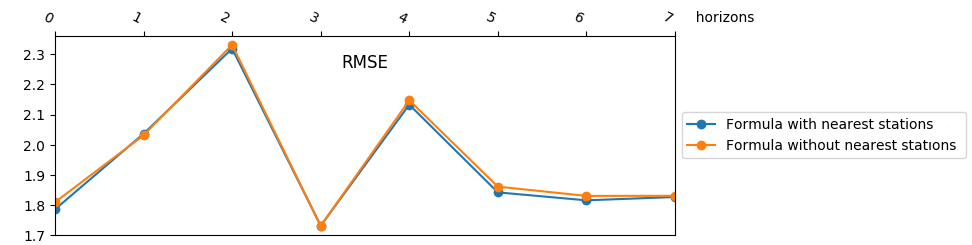
\includegraphics[width=\linewidth]{images/pic1_metrics_initial.png}
\caption{Модели, обученные на всех краткосрочных горизонтах -- Metrics for the 72-hours forecasts}
\label{pic1_metrics_initial}
\end{figure}


Было решено попробовать обучение отдельной модели только для первых семи часов. Тогда для всех строк в обучающей выборке модель будет знать показания с ближайших станций, благодаря чему эффект от этих данных должен повыситься. Чтобы не увидеть мнимое улучшение относительно базовой модели только за счёт того, что у усовершенствованной модели в обучающей выборке нет удалённых по времени наблюдений с меньшим качеством прогноза у поставщиков, сравнение проводилось с моделью без данных от ближайших станций, но обученной также только на первых 7 часах. Однозначного улучшения по метрикам также не получили, хотя фактор $fact1\_temperature\_delta$ стал вносить значительный вклад в ответ модели -- он оказался на 5 месте по эффекту, наравне с прогнозами температуры от поставщиков.

We decided to try to train a separate model only for the first seven hours. Then, for all the rows in the training sample, the model will know the readings from the nearest stations, so that the effect of these data should increase. In order not to see the supposed improvement with respect to the base model only because the improved model in the training sample does not have distant in time observations with a lower forecast quality from suppliers, the comparison was made with the model without data from the nearest stations, but trained also only at the first 7 hours. We also did not receive a strong improvement in metrics, although the factor $fact1\_temperature\_delta$ began to make a more significant contribution to the model's response -- it was on the 5th place in list of features, ordered by effect on model's answer, along with temperature forecasts from suppliers.

% метрики из https://st.yandex-team.ru/WEATHER-9187#1512471399000, без картинки
% про fstr Лана написала https://st.yandex-team.ru/WEATHER-9187#1512585426000

Далее были испробованы другие ограничения на число часов, которым ограничивается действие прогноза в будущее, хотелось найти баланс между сокращением применимости модели и улучшением метрик. По результатам экспериментов было выбрано ограничение в 3 часа от момента генерации прогноза. Далее прогнозы полученной модели были нарисованы на карте, чтобы увидеть, как они будут выглядеть для пользователя.

Further, we tried other restrictions on the number of hours that the forecast is limited to the future. We wanted to find a balance between reducing the applicability of the model and improving the metrics. Based on the results of the experiments, a restriction was chosen in 3 hours from the moment of generation of the forecast. Next, the predictions of the model were drawn on the map to see how they would look to the user.
% метрики https://st.yandex-team.ru/WEATHER-9187#1513066306000, странный пик

\begin{figure}
\centering
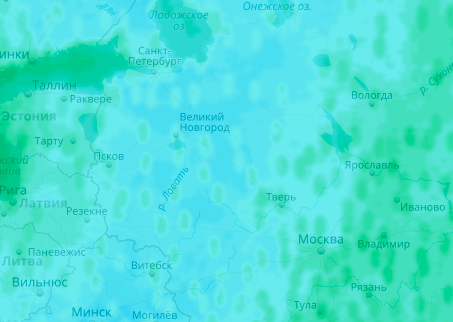
\includegraphics[width=0.7\linewidth]{images/pic2_map.png}
\caption{Пятна вокруг станций -- Stains around stations}
\label{pic2_map}
\end{figure}

На карте были обнаружены пятна вокруг станций, поставляющих данные (Рис.~\ref{pic2_map}). Они демонстрируют, что раз $temperature\_delta$ с ближайшей станции имеет большой вклад в прогноз модели, то на границе, после которой станция перестаёт считаться ближайшей, и данные от неё для модели пропадают, видны различия в прогнозе.


We can see on the map stains around the stations supplying the data (Fig.~\ref{pic2_map}). They demonstrate that since $temperature\_delta$ from the nearest station makes a big contribution to the model forecast, the differences in the forecast are seen on the border, after which the station ceases to be considered the nearest one, and the data from it for the model disappear.


\subsection{Расстояние до ближайших станций -- Distance to the nearest stations}

\begin{figure}
\centering
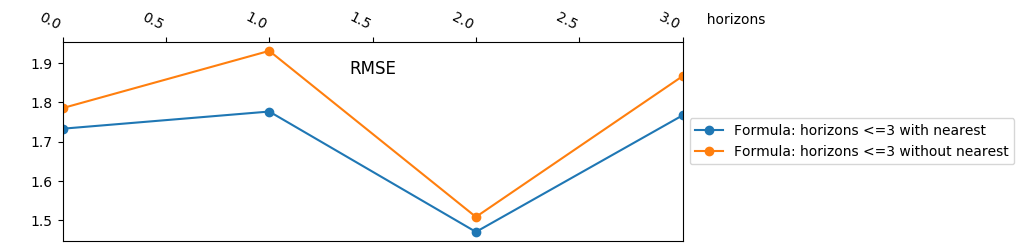
\includegraphics[width=\linewidth]{images/pic3_metrics_final.png}
\caption{Модель с использованием расстояний до ближайших станций}
\label{pic3_metrics_final}
\end{figure}

Для решения проблемы с пятнами было решено использовать простое сглаживание данных от ближайших станций, чтобы на границе их присутствия не было резкого скачка в значениях. Кроме этого в данные для обучения были добавлены расстояния от точки прогноза до ближайших станций, но по результатам экспериментов они не оказались полезны для модели.

To solve the problem with stains, we decided to use some smoothing of data from the nearest stations, so that there is no sharp jump in values at the border of their presence. In addition, distances from the prediction point to the nearest stations were added to the training data, but they proved useless for the model.

Для сглаживания был взят прогноз самого точного из наших поставщиков, которым подменялись значения с ближайших станций за пределами радиуса их использования ($max\_distance$). Далее для каждого наблюдения для двух ближайших станций были вычислены такие значения: 
\begingroup
\setlength\abovedisplayskip{0pt}
\begin{multline*}
smoothed\_fact\_temperature\_delta := \\\left\{
                \begin{array}{ll}
                  fact \cdot (1 - \frac{dist}{max\_distance}) + forecast \cdot \frac{dist}{max\_distance},\\\indent \text{     if }dist \le max\_distance  \\
                  forecast, \text{ if } dist > max\_distance
                \end{array}
              \right.,
\end{multline*}
\endgroup
\indent где $fact$ -- исходное значение с одной из ближайших станций, $dist$ -- расстояние до неё, а $forecast$ -- прогноз поставщика для точки, где она находится, на момент $time$.

[не хочу формулу перебивать в word] To smooth out the forecast the most accurate of our suppliers was taken. We replaced the values from the nearest stations outside the radius of their use ($max\_distance$) with forecast of this supplier. Further, for each observation we calculated smoothed value: inside the $max\_distance$ radius we took sum of $fact\_temperature\_delta$ and $forecast\_temperature\_delta$ with weights proportional to the distance to the station; outside the $max\_distance$ radius we took clean $forecast\_temperature\_delta$ values. 


С таким сглаживанием получили модель, которая показывает лучшие метрики, чем модель, обученная также на первых трёх часах, но без показаний с ближайших станций (Рис.~\ref{pic3_metrics_final}), и при этом не даёт пятен на картах. Сглаженные температуры с двух ближайших станций оказались на 1 и 4 местах по влиянию на ответ модели.

With this smoothing, we got a model that shows the better metrics than the model trained also at the first three hours, but without data from the nearest stations (Fig.~\ref{pic3_metrics_final}), and it doesn't make spots on the maps. The smoothed temperatures from the two nearest stations appeared on 1 and 4 places by influence on the model response.

% из графа https://nirvana.yandex-team.ru/flow/47895a5f-63eb-414e-9d80-ab7a45f32724/c601ecaa-a10a-42de-8675-9a5961681231/graph/FlowchartBlockOutput/4c8db20a-7836-46bd-b64c-6a812e8dc488
% чего-то очень большое улучшение



% У заключения нет номера главы
\section*{Заключение}
При работе над этой задачей было показано, что данные с ближайших станций могут помочь улучшить прогноз температуры.  Использовать их нужно с некоторым сглаживанием, чтобы не получить ярко выраженных окрестностей вокруг станций.

While working on this task, we proved the assumption that data from nearby stations can help to improve the temperature forecast.  We also found out that it's better to use them with smoothing, in order to not obtain distinct neighborhoods around the stations.

Эти изменения уже добавлены в продукт Яндекс.Погода и используются на постоянной основе в продакшене.

These changes have already been added to the Yandex.Weather and used on an ongoing basis in production.


В качестве возможных направлений развития этой задачи перечислю следующие:
\begin{itemize}
    \item использовать ближайшие станции для предсказания не только $temperature\_delta$, но и других показателей;
    \item использовать кросс-валидацию, чтобы уменьшить влияние конкретного разбиения на обучающую и тестовую выборки и более объективно оценивать изменения;
    \item поэкспериментировать с параметрами градиентного бустинга, по первым шагам в этом направлении похоже, что возможны значительные улучшения (Рис.~\ref{pic4_params});
    \item попробовать другие способы сглаживания показаний со станций по мере удаления точки прогноза от них. 
\end{itemize}


As possible directions of development of this task the following can be listed:
\begin{itemize}
    \item use nearest stations to predict not only $temperature\_delta$, but also other weather parameters;
    \item use cross validation to reduce the impact of a particular split to the training and test samples and evaluate changes more objectively;
    \item experiment with gradient boosting parameters, the first steps in this direction seem to be possible significant improvements;
    \item try other ways to smooth the readings from stations as you distance the prediction point from them. 
\end{itemize}



% картинка из https://nirvana.yandex-team.ru/flow/47895a5f-63eb-414e-9d80-ab7a45f32724/79a0c479-4853-4e40-a8a1-3dcba92479c4/graph
\begin{figure}
\centering
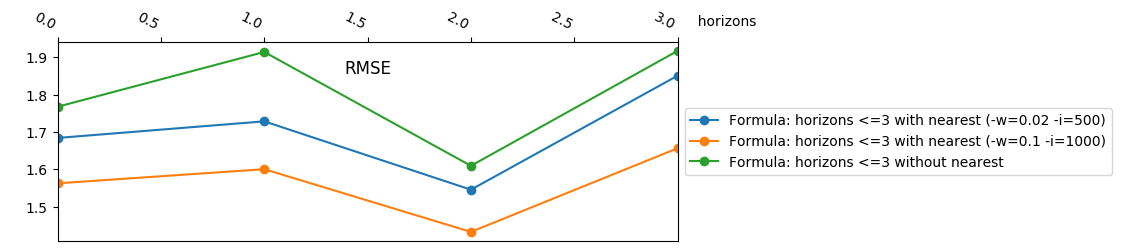
\includegraphics[width=\linewidth]{images/pic4_params.png}
\caption{Эксперимент с параметрами алгоритма Matrixnet -- в статье не будет}
\label{pic4_params}
\end{figure}


\setmonofont[Mapping=tex-text]{CMU Typewriter Text}
\bibliographystyle{ugost2008ls}
\bibliography{diploma.bib} 
\end{document}
